\documentclass[MasterThesisMain.tex]{subfiles}
\begin{document}
\chapter{Discussion}

\section{Experimental setup}
The experimental setup can be used in two ways. The first way with the optical fibre in the single point stage and the second way in the solvent vapour annealing chamber. When the optical fibre is fitted into the solvent vapour annealing chamber, the light must pass through a sapphire lens. This causes a great deal of reflected of light and effects the reflectance measurements taken. This can be seen by holding the static measurements seen in table \ref{tab:polymers} against the first fitted thickness values found in the figures for each polymer in chapter \ref{ch:results}. The effects may be small at the beginning of the solvent vapour annealing when the polymer has not swelled, but during swelling the reflectance measurement drops and can be zero in wavelength intervals. The sapphire lens effectively increases the dark measurement and when calculating the reflectance, since the dark measurement is in the denominator, lowers the reflectance measurements. If the thin film measurement decreases during the swelling this will also impact the reflectance measurement, lowering it even more. It can be seen when plotting the reflectance measurements alone with no strict axis interval that some reflectance measurements drops below zero, figure \ref{fig:drop}, the reason for this is unknown and close to zero, figure \ref{fig:drop2}. The dark measurements are taken when the optical fibre is fitted into the solvent vapour annealing chamber with a piece of black fabric where the wafer would lay. The black fabric is a piece of black cotton which has been taken from a bit of clothing. The effect, if there is any, of the black fabric has not been investigated. The distance from the wafer to the optical fiber is important, as it is seen to shift the whole reflectance measurement up and down the y axis. Up if the distance increases and down if it decreases. It is therefore very important to use a step wafer where the thickness is known to adjust the single point stage before a static measurement of a wafer with a thin film. When the optical fiber is placed in the solvent vapour annealing chamber the distance between the optical fiber and the wafer is much greater than it intended thus the sapphire lens is used to focus the light to illuminate the wafer. Calibrating the solvent vapour annealing setup is impossible at this point since the chamber is not big enough for the step wafer to be place in the chamber. Taking the best reference and dark measurement is key to a good reflectance measurement for the thin film, though it seems that the best measurement is impossible, it seems that a measurement close to good can be achieved as seen in the fitting of the fresnel equations using the homopolymer reflectance data.

\begin{figure}[H]
\centering
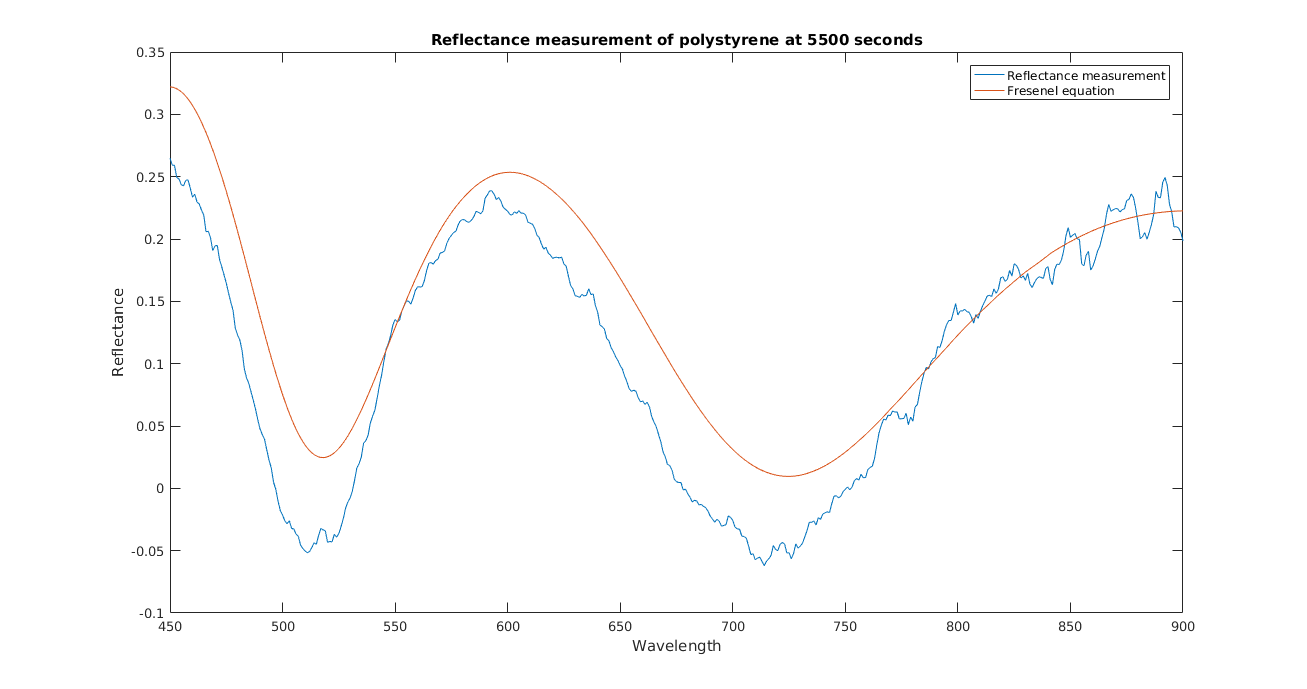
\includegraphics[width = \textwidth]{refldrop.png}
\caption{}
\label{fig:drop}
\end{figure}

\begin{figure}[H]
\centering
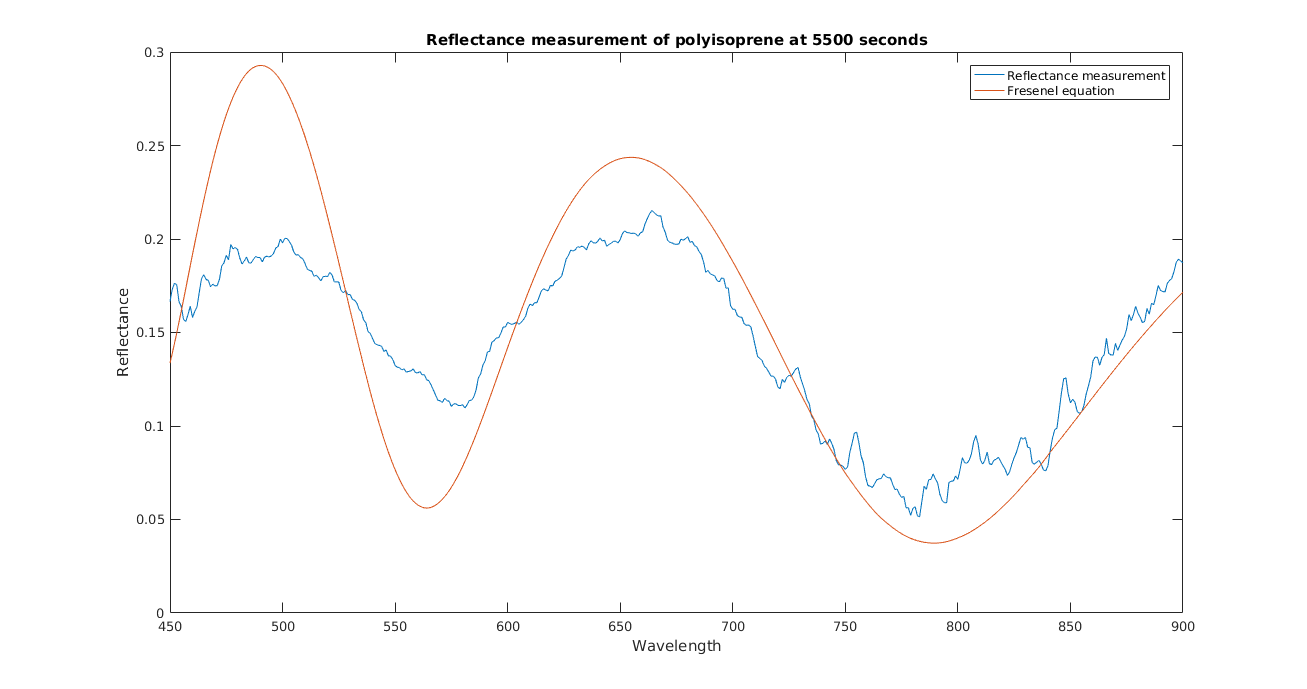
\includegraphics[width = \textwidth]{refldrop2.png}
\caption{}
\label{fig:drop2}
\end{figure}

\section{Refractive index dispersion of polymers and absorption}
The refractive index dispersion of the polymers has been shown in figure \ref{fig:dispshort} using the values given by the experimental method ellipsometry. It can be seen that the refractive index varies across the wavelengths. Polystyrene's refractive index does not vary as greatly as polyisoprene and the linear diblock copolymer polystyrene-b-polyisoprene. The fitting has not taken into account the dispersion of the refractive index, instead the constant refractive index has been used. It is unknown how the uptake of the solvent would effect the dispersion and how the dispersion would effect the reflectance measurements. An analytical study of the fresnel equations would be needed to fully grasp how changing the refractive indices impact the reflectance curves. Absorption is another parameter that can affect the reflectance measurements. Absorption is not present in the fresnel equations can can be the cause for the divergence between the reflectance measurements and the fresnel equations. 

\section{Refractive index of toluene vapour}   


\section{Mean square error fitting}
The mean square error fitting has been used as it was the fitting protocol used in the nano-calc software and other fitting methods have not been studied or implemented. The interval of fitting has been chosen to run from $\SI{450}{\nano\meter}$ to $\SI{900}{\nano\meter}$. This interval has been the easiest to fit to due to the reflectance measurements being smooth in this region and features present in this interval to fit. The fitting of the reflectance measurements follow the features seen in the fresnel equation but when swelling commences the reflectance measurements shift and drop. This can be seen in the figures \ref{fig:drop} and \ref{fig:drop2}. Both figures have been taken at the $5500$ second mark, at the end of the max swelling interval and the reflectance measurements have shifted and dropped with respect to the theoretical model. The way the fitting has been implemented into matlab can also be critiqued. The fitting loads a reflectance measurements and loops through the refractive indices for air and the thin film and the thickness values. For polystyrene this amounted to $13,380,120$ combinations taking roughly $75$ minutes to loop through, for polyisoprene $8,116,164$ combinations taking roughly $44$ minutes and polystyrene-b-polyisoprene $2,462,592$ combinations roughly $13$ minutes. The fitting on the two homopolymers shown results that are in tune with what is expected. As the nitrogen through the toluene solvent, the vapour in the chamber increases and the refractive index for the ambient increases. It can be also said for the thin films refractive index as we expect solvent uptake and this can also be seen in the thickness values increasing. The ambient refractive index is normally set to $1$ when making static measurements but the fitting of the reflectance measurements in the ambient study shows that the reflectance measurements decreases during swelling and increasing the refractive index for the ambient fits the fresnel reflectance equations well. The increases in the mean square error values for the ambient study can be caused by the large step sizes in the refractive index. The step size used in the  fitting have been set crudely. The step size for the thickness is set to $1$. Since we are working on the nanoscale, having thickness values with decimals does not shine light on anything interesting when looking at the thickness measurements. The step size for both refractive indices has been set to $0.1$. This has been set to one decimal for two reasons. The first reason is that more values the fitting has to loop through the long the fitting will take, and the second reason is that a finer step size would not contribute useful information to the thickness fitting.        

\section{Solvent vapour annealing}

In the solvent vapour annealing protocol the nitrogen flow has been set to be constant through out the protocol. The assumption is holding the flow constant will hold the vapour pressure in the chamber constant. This is a crude assumption since the variables flow and pressure are heavily dependant on tube sizing, the volume of the solvent vapour annealing chamber, the volume of the bubbler and the volume of liquid present in the bubbler. Taking these variable into account and calculating the vapour pressure constitutes research project in itself. The solvent vapour annealing protocol has been programmed into a script which the mass flow controllers could read and run. As seen in figure \ref{fig:slowslow}, the increases and decreases of flow controlled by the mass flow controllers happen at a fraction of time before they should. Each step apart from the maximum swelling should have a length of $1000$ seconds. The solvenet vapour annealing time was not saved, so i can not precisely determine when the mass flow controllers changed the flow but the solvent vapour annealing protocol was close to what was scripted.   

\section{Polystyrene and Polyisoprene}
When fitting the fresnel equations onto solvent vapour annealing data, the homopolymers results behaved as anticipated but the diblock copolymer results were the opposite to what was expected. The expected result was an increase in ambient refractive index and thin film refractive index which coincided with the increase of toluene vapour present in the chamber. What i expected with the thickness results was an increase in thickness starting every time there was an increase of toluene vapour. The thickness result shows a 'shark dorsel fin' during the maximum swelling region. One can think that if the maximum swelling was left the thickness would reach a constant value. There is an interval of time between a change from the mass flow controllers to the beginning of a change in the polymers, this is called a response time. [ADD Values]. The mean square error for both the polystyrene and polyisoprene show a constant mean square error expect for when the maximum swelling commences. This is because of the fit and the reflectance data not matching up. In figure \ref{fig:drop} it can be seen that the fit for polystyrene is higher than the polystyrene reflectance measurement. In figure \ref{fig:drop2} the amplitude of the polyisoprene fit is much greater that the polyisoprene reflectance measurement. During the swelling it is apparent that something is happening that the fresnel equations does not accommodate for. This could be a multitude of things since the fresnel equations are simple. The fresnel equations do not account for an inhomogeneous increase in thickness. The roughness, variation of thickness in the thin film, can play a role as this can cause diffusive reflection and decrease the reflectance measurements. A reflectance measurement is taken every 10 seconds   

\section{Polystyrene-b-polyisoprene}
The fitting for the diblock copolymer polystyrene-b-polyisoprene behaves strangely. The fitting showed an ambient refractive index starting at $1.2$ and decreasing in value as the toluene vapour increased. The thin film refractive index does not increase until the solvent vapour annealing protocol reaches the region of maximum swelling. In this region the thin film refractive index climbs rapidly and is erratic throughout the maximum swelling. The thickness does increase nicely through out the solvent vapour annealing protocol. The mean square error is large at the start of the swelling and decreases during the swelling. The mean square error does peak during the swelling, this coincides with the fitting protocol changing the ambient refractive index from $1$ to $1.1$. The fitting implemented has used one layer with a varying real refractive index. This simple model does not capture the actual structure seen with diblock copolymers. Diblock copolymers organises itself into a multilayer system consisting of a layer of one end of the polymer with the other end forming the next layer, an A-B-A-B thin film structure, which can consist of many layers. This structure is not seen in the homopolymers as they consist of one monomer repeated. Fitting for this multilayer thin film with my fitting protocol requires a large amount of computer power. When adding a new variable into the protocol, you are effectively multiplying the amount of values the new variable can have onto the amount of combination the fitting protocol, increasing the total amount of calculations the fitting protocol has to calculate. The fitting protocol is not suited to diblock copolymers.     




\end{document}